%Manual técnico

\section{Introducción}
\begin{Large}$\mathbf{E}$\end{Large}l artículo periodístico o noticia, es la información de un hecho de interés ocurrido en un periodo de tiempo determinado. Constituye el elemento primordial en la información de la prensa y del género básico del periodismo \citep{CU1}. Conocer los acontecimientos del mundo independientemente del tema, día o lugar en el cual se han suscitado, tiene una gran importancia en la sociedad, se comparten por distintos medios de comunicación, tales como la televisión, redes sociales, diarios, blogs y la radio. Nos permiten conocer la situación económica del país, logros de la ciencia, desastres naturales, la situación en cuestión de inseguridad entre otros hechos. En el ámbito de las inversiones, crean expectativas y eso a su vez puede modificar los planes de inversión en cualquier sector, siendo así de suma importancia compartirlas de una forma eficaz \citep{CU2}.\\

El uso de páginas web como medio de comunicación está en incremento, permitiendo consultar noticias de distintos sitios como los periódicos electrónicos; su información al igual que un diario tradicional se encuentra dividida en secciones para facilitar la consulta, sin embargo, la clasificación suele variar en cada portal, incluso teniendo el mismo contenido. Un problema mayor se encuentra en los sitios independientes, los cuales no cuentan con una segmentación particular, haciendo difícil realizar una búsqueda eficaz.\\

\section{Objetivo}
Recolectar y clasificar noticias de acuerdo a su contenido y periodo de publicación, las noticias que satisfagan ambos filtros serán mostradas.

\section{Objetivos específicos}
\begin{itemize}
  \item Obtener información de diferentes fuentes como diarios, sitios de noticias, blogs y foros
  \item Analizar de forma automática el contenido de las noticias para satisfacer los filtros establecidos por el usuario
  \item Mostrar las noticias que cumplieron con los filtros establecidos, así como su enlace (URL) para redirigirlos a la página de la noticia
\end{itemize}

\section{Instalación}

	El presente sistema web ha sido desarrollado bajo el sistema operativo \textit{Ubuntu} en su versión 18.04.3, las siguientes bibliotecas serán instaladas utilizando la terminal del sistema operativo, son necesarias para el correcto funcionamiento del sistema
	\subsection{Recolector}
	El recolector ha sido construido bajo el lenguaje de programación \textit{Python} utilizando el framework \textif{Scrapy} el cual se utiliza para recuperar información de diversos sitios, para su instalación se utiliza el siguiente comando:
	\begin{lstlisting}[language=bash]
  		$ pip3 install Scrapy
	\end{lstlisting}

	\subsection{Clasificador}
	El clasificador ha sido programado bajo el lenguaje de programación \textit{Python}, previó a llevar a cabo el proceso de clasificación, se procede a realizar dos tareas importantes, tokenizar y lematizar; para realizar estas tareas se ha utilizado la biblioteca \textit{Spacy}, para su instalación se utiliza el comando:
	\begin{lstlisting}[language=bash]
  		$ pip3 install -U spacy
  		$ python -m spacy download es_core_news_sm
	\end{lstlisting}

	Para el clasificador se ha utilizado la biblioteca \textit{Scikit Learn}, para su instalacións se utiliza el siguiente comando:
	\begin{lstlisting}[language=bash]
		$ pip3 install -U scikit-learn
	\end{lstlisting}

	\subsection{Aplicación Web}
	La presente aplicación Web ha sido desarrollada bajo el lenguaje de programación \textit{Java} es necesario instalar NetBeans en su versión 8.2, en la siguiente liga \textit{https://netbeans.org/downloads/8.2/} se encuentra la versión 8.2, debido a que se realiza una aplicación web es necesario instalar la versión \textit{Java EE} la cual incluye \textit{Apache TomCat}.
	\\
	Una vez que se ha descargado NetBeans nos ubicamos en la carpeta donde se haya descargado nuestro archivo y ejecutamos el siguiente comando:
	\begin{lstlisting}[language=bash]
		$ chmod +x netbeans-8.2-javaee-linux.sh 
		$ -/netbeans-8.2-javaee-linux.sh 
	\end{lstlisting}

	Una vez instaladas todas las bibliotecas previas, es necesario ubicarnos en la siguiente carpeta:
	\begin{lstlisting}[language=bash]
		/ApplicacionWeb/TT2/web/resources/Recolector$
	\end{lstlisting}
	Una vez ubicados en dicha carpeta ejecutaremos el siguiente comando:
	\begin{lstlisting}[language=bash]
		$ scrapy startproject TT2
	\end{lstlisting}
	
\section{Ejecución}
Una vez finalizada la instalación y creación del recolector, se procederá a abrir NetBeans, una vez ingresado se procederá a abrir el proyecto, como se muestra en la Figura \ref{fig:seleccionarProyecto}
\begin{figure}[H]
	\centering
	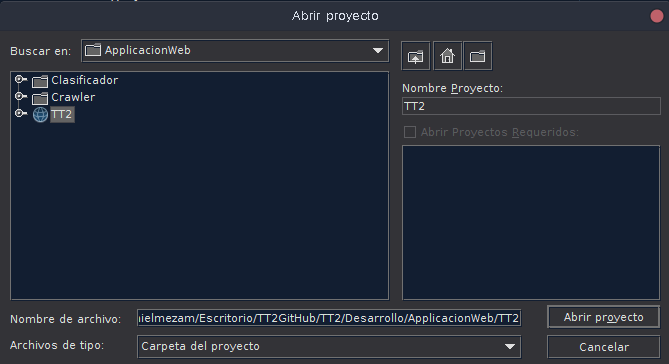
\includegraphics[scale=0.6]{imagenes/abrirProyecto.png}
	\caption{Se selecciona el proyecto TT2}
	\label{fig:seleccionarProyecto}
\end{figure}

Una vez abierto el proyecto se ejecutará el sistema, dando click derecho sobre el archivo \textit{inicio.xhtml} y seleccionando la opción ejecutar, el archivo se muestra en la Figura \ref{fig:inicio}

\begin{figure}[H]
	\centering
	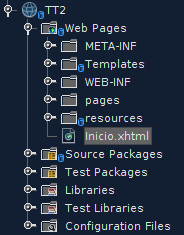
\includegraphics[scale=0.6]{imagenes/ejecutar.png}
	\caption{Se ejecuta el archivo inicio.xhtml}
	\label{fig:inicio}
\end{figure}